After confirming that the operational amplifier circuit was functioning
correctly, students built the circuit in Figure~\ref{fig:weinBridgeSchem},
using resistors of size~\SI{10}{\kilo\ohm} for all elements except~$R_3$, which
was represented by a~\SI{25}{\kilo\ohm} potentiometer.  The specific value
of~$R_4$ was measured on the in-lab digital voltage meters, allowing students
to tune~$R_3$ to exactly twice the value of~$R_4$ via the same meter.  While it
was not possible to dynamically tune the capacitance to a required value,
students used an assortment of capacitor combinations to create a balanced pair
of elements as near the calculated~\SI{4.822}{\nano\farad} as possible.

Once constructed, the output of the circuit was monitored on an oscilloscope.
It was expected to not be functioning properly, so the value of~$R_3$ was
adjusted further until an accurate sine waveform was produced.  The resulting
output with a correctly-tuned system is shown in Figure~\ref{fig:goodShot}.
%
\begin{figure}[H]
	\centering
	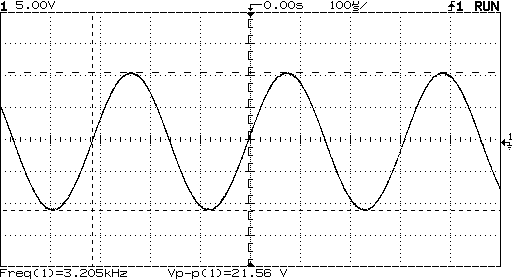
\includegraphics[width=.6\textwidth]{img/shot/pt2shot.png}
	\parbox{.6\textwidth}{
	\caption[Oscilloscope Screenshot --- Functioning System]{Oscilloscope
	screenshot of a correctly-tuned sine wave generator, based on the system
	shown in Figures~\ref{fig:blockDiag} and~\ref{fig:weinBridgeSchem}.  Note
	the frequency of~\SI{3.205}{\kilo\hertz}, which is just~\SI{2.87}{\percent}
	below the expected value.}
	\label{fig:goodShot}}
\end{figure}
%
The output voltage was measured peak-to-peak to be~\SI{21.56}{\volt}, below the
logical upper-limit of the~\SI{25}{\volt} supply.  Similarly, the output
frequency was just below the~\SI{3.3}{\kilo\hertz} frequency for which the
system was designed at~\SI{3.205}{\kilo\hertz}  By using~\eqref{eq:frequency}
with the average of the measured values, the expected frequency was
re-calculated:
%
\begin{align*}
	R_\text{avg} &= \frac{R_1 + R_2 + R_4}{3}
	             = \frac{\SI{9.97}{\kilo\ohm} + \SI{9.96}{\kilo\ohm} + \SI{9.95}{\kilo\ohm}}{3}
				 = \SI{9.96}{\kilo\ohm}\\
	C_\text{avg} &= \frac{C_1 + C_2}{2}
				 = \frac{\SI{4.839}{\nano\farad} + \SI{4.808}{\nano\farad}}{2}
				 = \SI{4.823}{\nano\farad}
\end{align*}
thus
\begin{equation*}
	f_0 = \frac{1}{2 \pi R_\text{avg} C_\text{avg}}
		= \frac{1}{2 \pi (\SI{9.96}{\kilo\ohm}) (\SI{4.823}{\nano\farad})}
		= \SI{3.312}{\kilo\hertz}
\end{equation*}
%
Because this value is so close to the designed value, it is clear that the
aforementioned element variance had only a very minor effect on the output
frequency.  In fact, students subsequently varied the resistance across the
potentiometer~$R_3$ to monitor its contribution to the output waveform.
Oscilloscope screenshots were captured when the potentiometer was adjusted both
higher and lower than its correctly-tuned resistance of~\SI{20.149}{\kilo\ohm},
and can be seen in Figure~\ref{fig:badPotShots}.
%
\begin{figure}[H]
	\centering
	\subfloat[Potentiometer too low]{\label{fig:badPotLow}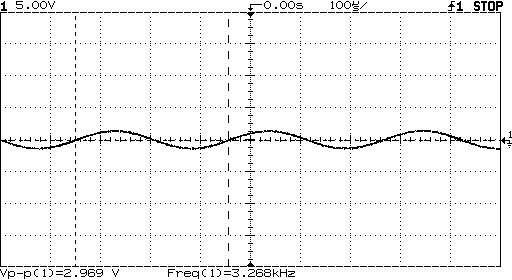
\includegraphics[width=.4\textwidth]{img/shot/pt3lowShot.png}}
	\quad
	\subfloat[Potentiometer too high]{\label{fig:badPotHigh}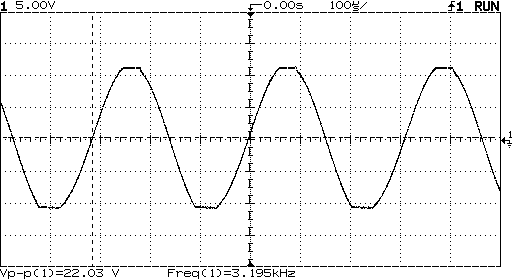
\includegraphics[width=.4\textwidth]{img/shot/pt3hiShot.png}}

	\parbox{.8\textwidth}{
	\caption{Output of two improperly-tuned~$R_3$ potentiometers.  Note in the
	case of~\subref{fig:badPotLow} that the output only momentarily looks like
	this, as it becomes simply noise soon after.  Also note the clipping that
	occurs in~\subref{fig:badPotHigh}.}
	\label{fig:badPotShots}}
\end{figure}
%
When the potentiometer was tuned too low, the output amplitude shrinks very
quickly to merely noise, resembling only momentarily the wave shown in
Figure~\ref{fig:badPotLow}.  When the potentiometer was tuned too high as in
Figure~\ref{fig:badPotHigh}, a wave of proper frequency was created, but the
waveform became clipped due to the limited supply voltage.

Much as it was important in experiment three for the voltage regulator to
function properly at different source voltages, it is equally important for the
sine wave generator to create a usable signal for varying sources.  This was
tested by varying the opamp's DC power supply voltage~(shown as a
static~\SI{25}{\volt} in Figure~\ref{fig:weinBridgeSchem}'s schematic)
from~\SI{30}{\volt} down to~\SI{5}{\volt} and monitoring the effects of the
output frequency and voltage.  Results of this voltage sweep are shown in
Table~\ref{tab:vSweepData} and Figure~\ref{fig:vSweepPlot}.
%
\begin{table}[H]
	\centering
	\begin{tabular}{|c|c|c|}
	\hline
	$\boldsymbol{V_\mathrm{PS}}$ \tbf{(\si{\volt})} &
		$\boldsymbol{V_\mathrm{P-P}}$ \tbf{(\si{\volt})} &
			$\boldsymbol{f}$ \tbf{(\si{\kilo\hertz})} \\ \hline
	30		& 26.41		& 3.205 \\ \hline
	25		& 21.56		& 3.210 \\ \hline
	20		& 16.88		& 3.236 \\ \hline
	15		& 12.05		& 3.226 \\ \hline
	10		& 7.344		& 3.231 \\ \hline
	5		& 2.656		& 3.273 \\ \hline
\end{tabular}
\\
	\parbox{.6\textwidth}{
	\caption[Voltage Sweep Data]{Data recorded from the voltage sweep,
		measuring the peak-to-peak voltage~($V_\mathrm{P-P}$) and
		frequency~($f$) on an oscilloscope as a function of the power supply
		voltage~($V_\mathrm{PS}$).}
	\label{tab:vSweepData}}
\end{table}
%
This data shows that regardless of the input voltage, the output frequency will
remain roughly unchanged, increasing just~\SI{0.68}{\kilo\hertz} over the
course of the voltage sweep, or~\SI{-0.027}{\kilo\hertz\per\volt}.
%
\todo[inline]{Explain voltage sweep results}
\begin{figure}[H]
	\centering
	\begin{tikzpicture}[gnuplot]
%% generated with GNUPLOT 4.4p2 (Lua 5.1.4; terminal rev. 97, script rev. 96a)
%% Sat 15 Oct 2011 11:14:53 PM EDT
\gpsolidlines
\gpcolor{gp lt color axes}
\gpsetlinetype{gp lt axes}
\gpsetlinewidth{1.00}
\draw[gp path] (1.320,0.985)--(8.830,0.985);
\gpcolor{gp lt color border}
\gpsetlinetype{gp lt border}
\draw[gp path] (1.320,0.985)--(1.500,0.985);
\node[gp node right] at (1.136,0.985) { 0};
\gpcolor{gp lt color axes}
\gpsetlinetype{gp lt axes}
\draw[gp path] (1.320,1.529)--(8.830,1.529);
\gpcolor{gp lt color border}
\gpsetlinetype{gp lt border}
\draw[gp path] (1.320,1.529)--(1.500,1.529);
\node[gp node right] at (1.136,1.529) { 5};
\gpcolor{gp lt color axes}
\gpsetlinetype{gp lt axes}
\draw[gp path] (1.320,2.072)--(8.830,2.072);
\gpcolor{gp lt color border}
\gpsetlinetype{gp lt border}
\draw[gp path] (1.320,2.072)--(1.500,2.072);
\node[gp node right] at (1.136,2.072) { 10};
\gpcolor{gp lt color axes}
\gpsetlinetype{gp lt axes}
\draw[gp path] (1.320,2.616)--(1.504,2.616);
\draw[gp path] (3.892,2.616)--(8.830,2.616);
\gpcolor{gp lt color border}
\gpsetlinetype{gp lt border}
\draw[gp path] (1.320,2.616)--(1.500,2.616);
\node[gp node right] at (1.136,2.616) { 15};
\gpcolor{gp lt color axes}
\gpsetlinetype{gp lt axes}
\draw[gp path] (1.320,3.159)--(1.504,3.159);
\draw[gp path] (3.892,3.159)--(8.830,3.159);
\gpcolor{gp lt color border}
\gpsetlinetype{gp lt border}
\draw[gp path] (1.320,3.159)--(1.500,3.159);
\node[gp node right] at (1.136,3.159) { 20};
\gpcolor{gp lt color axes}
\gpsetlinetype{gp lt axes}
\draw[gp path] (1.320,3.703)--(8.830,3.703);
\gpcolor{gp lt color border}
\gpsetlinetype{gp lt border}
\draw[gp path] (1.320,3.703)--(1.500,3.703);
\node[gp node right] at (1.136,3.703) { 25};
\gpcolor{gp lt color axes}
\gpsetlinetype{gp lt axes}
\draw[gp path] (1.320,4.246)--(8.830,4.246);
\gpcolor{gp lt color border}
\gpsetlinetype{gp lt border}
\draw[gp path] (1.320,4.246)--(1.500,4.246);
\node[gp node right] at (1.136,4.246) { 30};
\gpcolor{gp lt color axes}
\gpsetlinetype{gp lt axes}
\draw[gp path] (1.320,4.790)--(8.830,4.790);
\gpcolor{gp lt color border}
\gpsetlinetype{gp lt border}
\draw[gp path] (1.320,4.790)--(1.500,4.790);
\node[gp node right] at (1.136,4.790) { 35};
\gpcolor{gp lt color axes}
\gpsetlinetype{gp lt axes}
\draw[gp path] (1.320,0.985)--(1.320,4.790);
\gpcolor{gp lt color border}
\gpsetlinetype{gp lt border}
\draw[gp path] (1.320,0.985)--(1.320,1.165);
\node[gp node center] at (1.320,0.677) { 0};
\gpcolor{gp lt color axes}
\gpsetlinetype{gp lt axes}
\draw[gp path] (2.572,0.985)--(2.572,2.425);
\draw[gp path] (2.572,3.349)--(2.572,4.790);
\gpcolor{gp lt color border}
\gpsetlinetype{gp lt border}
\draw[gp path] (2.572,0.985)--(2.572,1.165);
\node[gp node center] at (2.572,0.677) { 5};
\gpcolor{gp lt color axes}
\gpsetlinetype{gp lt axes}
\draw[gp path] (3.823,0.985)--(3.823,2.425);
\draw[gp path] (3.823,3.349)--(3.823,4.790);
\gpcolor{gp lt color border}
\gpsetlinetype{gp lt border}
\draw[gp path] (3.823,0.985)--(3.823,1.165);
\node[gp node center] at (3.823,0.677) { 10};
\gpcolor{gp lt color axes}
\gpsetlinetype{gp lt axes}
\draw[gp path] (5.075,0.985)--(5.075,4.790);
\gpcolor{gp lt color border}
\gpsetlinetype{gp lt border}
\draw[gp path] (5.075,0.985)--(5.075,1.165);
\node[gp node center] at (5.075,0.677) { 15};
\gpcolor{gp lt color axes}
\gpsetlinetype{gp lt axes}
\draw[gp path] (6.327,0.985)--(6.327,4.790);
\gpcolor{gp lt color border}
\gpsetlinetype{gp lt border}
\draw[gp path] (6.327,0.985)--(6.327,1.165);
\node[gp node center] at (6.327,0.677) { 20};
\gpcolor{gp lt color axes}
\gpsetlinetype{gp lt axes}
\draw[gp path] (7.578,0.985)--(7.578,4.790);
\gpcolor{gp lt color border}
\gpsetlinetype{gp lt border}
\draw[gp path] (7.578,0.985)--(7.578,1.165);
\node[gp node center] at (7.578,0.677) { 25};
\gpcolor{gp lt color axes}
\gpsetlinetype{gp lt axes}
\draw[gp path] (8.830,0.985)--(8.830,4.790);
\gpcolor{gp lt color border}
\gpsetlinetype{gp lt border}
\draw[gp path] (8.830,0.985)--(8.830,1.165);
\node[gp node center] at (8.830,0.677) { 30};
\draw[gp path] (8.830,0.985)--(8.650,0.985);
\node[gp node left] at (9.014,0.985) { 0};
\draw[gp path] (8.830,1.529)--(8.650,1.529);
\node[gp node left] at (9.014,1.529) { 0.5};
\draw[gp path] (8.830,2.072)--(8.650,2.072);
\node[gp node left] at (9.014,2.072) { 1};
\draw[gp path] (8.830,2.616)--(8.650,2.616);
\node[gp node left] at (9.014,2.616) { 1.5};
\draw[gp path] (8.830,3.159)--(8.650,3.159);
\node[gp node left] at (9.014,3.159) { 2};
\draw[gp path] (8.830,3.703)--(8.650,3.703);
\node[gp node left] at (9.014,3.703) { 2.5};
\draw[gp path] (8.830,4.246)--(8.650,4.246);
\node[gp node left] at (9.014,4.246) { 3};
\draw[gp path] (8.830,4.790)--(8.650,4.790);
\node[gp node left] at (9.014,4.790) { 3.5};
\draw[gp path] (1.320,4.790)--(1.320,0.985)--(8.830,0.985)--(8.830,4.790)--cycle;
\node[gp node center,rotate=-270] at (0.246,2.887) {Output Voltage, $V_\mathrm{P-P}$ (V)};
\node[gp node center,rotate=-270] at (10.087,2.887) {Output Frequency, $f$ (kHZ)};
\node[gp node center] at (5.075,0.215) {Power Supply Voltage, $V_\mathrm{PS}$ (V)};
\node[gp node center] at (5.075,5.252) {Voltage Sweep: Output Voltage};
\draw[gp path] (1.504,2.425)--(1.504,3.349)--(3.892,3.349)--(3.892,2.425)--cycle;
\draw[gp path] (1.504,3.349)--(3.892,3.349);
\node[gp node right] at (2.608,3.041) {$V_\mathrm{P-P}$};
\gpcolor{gp lt color 0}
\gpsetlinetype{gp lt plot 0}
\gpsetlinewidth{3.00}
\draw[gp path] (2.792,3.041)--(3.708,3.041);
\draw[gp path] (8.830,3.856)--(7.578,3.329)--(6.327,2.820)--(5.075,2.295)--(3.823,1.783)%
  --(2.572,1.274);
\gpcolor{gp lt color border}
\node[gp node right] at (2.608,2.733) {$f$};
\gpcolor{gp lt color 1}
\gpsetlinetype{gp lt plot 1}
\draw[gp path] (2.792,2.733)--(3.708,2.733);
\draw[gp path] (8.830,4.469)--(7.578,4.475)--(6.327,4.503)--(5.075,4.492)--(3.823,4.498)%
  --(2.572,4.543);
\gpcolor{gp lt color border}
\gpsetlinetype{gp lt border}
\gpsetlinewidth{1.00}
\draw[gp path] (1.320,4.790)--(1.320,0.985)--(8.830,0.985)--(8.830,4.790)--cycle;
%% coordinates of the plot area
\gpdefrectangularnode{gp plot 1}{\pgfpoint{1.320cm}{0.985cm}}{\pgfpoint{8.830cm}{4.790cm}}
\end{tikzpicture}
%% gnuplot variables

	\parbox{4.25in}{
	\caption[Voltage Sweep Plot]{Plotted measurements from a supply voltage
	sweep.  The measured values from this test are in
	Table~\ref{tab:vSweepData}.  Note that the output voltage increases
	linearly with the supply voltage, while the frequency remains nearly
	constant.}
	\label{fig:vSweepPlot}}
\end{figure}
%
As is expected, the peak-to-peak voltage of the output signal decreases with
the supply voltage.  This is a direct result of the characteristics of an
operational amplifier, a device that outputs a voltage somewhere between its
two supply nodes ---~$V_\text{PS}$ and~0, in this case.  An oscilloscope
screenshot was captured for each step of the sween, some of which are shown in
the Appendix \todo{Add ref} of this document.

\todo[inline,color=green]{Multi-fig of plots: 30V, 15V, 5V in appendix}

The effects of an increase in resistance for resistor~$R_1$ were examined as
well.  Since this was a fixed-value element, its resistance was increased by
simply warming it between the student's fingers.  As its temperature (and thus
resistance) increased, the output voltage decreased by roughly~\SI{0.5}{\volt}
and the output signal's frequency increased by roughly~\SI{0.02}{\kilo\hertz}.
While these are not major changes, their existence shows the importance of
using stable and accurate resistors.
\missingfigure[figwidth=.6\textwidth]{part6 plots}


